\documentclass{article}
\usepackage{geometry}
 \geometry{
 a4paper,
 %total={170mm,257mm},
 left=20mm,
 top=15mm,
 right=15mm
 }
\usepackage[utf8]{inputenc}
\usepackage{cite}
\usepackage[colorlinks=true,linkcolor=blue]{hyperref}
\usepackage[spanish]{babel} % para que comandos como \today den el resultado en castellano
\usepackage{caratula2}
\usepackage{fancyhdr}
\usepackage{listings}
\usepackage{color}
\usepackage[pdftex]{graphicx}
\usepackage{float}
\usepackage{caption}
\usepackage{subcaption}
\usepackage{amsmath}
\usepackage{amssymb}
% Estos paquetes los agregé para poder escribir en pseudocódigo
\usepackage{algorithm}
\usepackage{url}
\usepackage[noend]{algpseudocode}
\usepackage{booktabs} % To thicken table lines
\usepackage{todonotes}
\makeatletter
\def\BState{\State\hskip-\ALG@thistlm}
\makeatother


\titulo{Trabajo Práctico 3}
\subtitulo{Cuadrados Mínimos Lineales}

\begin{document}

\fecha{\today}

\materia{Métodos Numéricos}
\submateria{2do Cuatrimestre de 2021}

\integrante{Olmedo, Dante}{195/13}{dante.10bit@gmail.com}
\integrante{Amigo, Martín}{362/17}{martinamigo@protonmail.com}
\integrante{Monasterio, Gonzalo}{153/18}{gonzamonas@gmail.com}
\integrante{Manusovich, Ariana}{262/20}{arimanuso@gmail.com}

\maketitle
\section{Palabras Clave}
\textbf{Cuadrados Mínimos Lineales, Regresión Lineal}

\tableofcontents
\newpage
\section{Resumen}
En el siguiente trabajo utilizamos el método de predicción de características conocido como Cuadrados Mínimos Lineales(CML) para analizar la predictibilidad de distintos features de nuestra base de datos, y probar las diferentes maneras con las que podemos mejorar nuestra estimación.
Se hizo un análisis exploratorio de los datos para identificar características propias de cada variable dándonos las bases para nuestro modelo y la elección de los regresores.
En las siguientes secciones presentamos los resultados e investigaciones que llevaron a concluir que un modelo que explique bien la expectativa de vida tiene que incluir variables económicas como el \textit{Income Composition of Resources} y el \textit{Percentage expenditure}, alguna variable sobre la vacunación infantil y alguna sobre la nutrición. Asimismo, la cantidad de muertes infantiles por VIH/SIDA y la cantidad de homicidios son indicadores a tener en cuenta.
También separamos al dataset en dos grandes categorías (Developed/Developing) para observar características propias de cada conjunto y encontrar regresores mas específicos para cada caso.

\newpage
\section{Introducción}
    La expectativa de vida de un determinado país es una métrica cuyo análisis es del interés de varias áreas y ramas de la ciencia y economía. En el análisis de inversiones la expectativa de vida puede decirnos algo sobre la salud de su población, la longevidad de los trabajadores y que tan proclives son a situaciones de riesgo como accidentes.
    Es de interés para el mercado inmobiliario pues la expectativa de vida de la población de un país puede cambiar el coste de la propiedad de manera substancial. Y del lado científico, entender los motivos detrás de la expectativa de vida da un indicador de problemas que aún no fueron atacados lo suficiente y podrían tener un gran impacto.
    
    En este sentido la predicción automática de dicho valor a partir de los datos recogidos por la OMS y, posiblemente aumentados con datos demográficos del área geográfica en que se encuentra, podría ser una solución ideal. Existen herramientas que nos permiten realizar estas predicciones, y así mismo la de cualquier otra variable para la cual deseemos estimar. 
    
    La herramienta en cuestión será un algoritmo de clasificación supervisado que entrenamos con un conjunto de datos de la OMS, que incluye la expectativa de vida, ya conocida. Una vez entrenado, evaluamos la calidad de la predicción con distintas métricas.
    
    El algoritmo sigue el método de cuadrados mínimos lineales\cite{MLS:qhe}, que dado un conjunto de pares ordenados (variables independientes y variable dependiente), intenta encontrar la función continua que dependa de las variables independientes, y que mejor se aproxime a la variable dependiente.
    
    Para evaluar la calidad de las predicciones realizadas, usaremos  \textit{Relative Standard Error} (RSE), \textit{R-Squared} (R2) y \textit{Adjusted R-Squared}(Adjusted R2) como métricas \cite{Met:qhe}.
    
    \subsection{Conjunto de datos}
    Para las experimentaciones contamos con un conjunto de datos de la OMS con las siguientes características:
    \begin{itemize}
     \item Country: País de donde vienen los demás datos, vale como ID.
     \item  Status: Variable categórica que se divide entre Developed o Developing.
     \item  Alcohol: Registrado per cápita para mayores de 15, en litros de alcohol puro.
     \item Mortalidad: Métricas acerca de la mortalidad de un grupo(Adult mortality, Infant deaths y under-five deaths, normalmente tomadas como porcentaje cada 1000 habitantes.
     \item Percentage expenditure: Porcentaje del PBI utilizado en salud.
     \item Enfermedad: varias características relacionadas con enfermedades(Porcentaje de inmunización de Hepatitis B,difteria y Polio en el primer año de edad, casos cada 1000 habitantes de Measles y muertes por VIH/SIDA en el primer año de edad).
     \item BMI: Índice de peso promedio de la población de un país entera.
     \item Métricas generales: GDP (PBI), Population, Income composition of resources(Índice de desarrollo humano en términos del manejo del gasto de recursos) y Schooling(años de educación).
     \item Thinness: Porcentaje de desnutrición separada entre las edades de 5 a 9, y 10 a 19.
    \end{itemize}
    
    La característica que intentamos predecir es la expectativa de vida, la cantidad en años que se espera viva una persona en promedio.
    \subsection{Cuadrados Mínimos Lineales}\label{sec:into_CML}
    El algoritmo de cuadrados mínimos lineales toma un conjunto de pares ordenados o mediciones ($x_{i},y_{i}$) con $0\leq i\leq m$ (En nuestro caso $x_{i}$ es un vector fila en el que cada columna representa una característica para un país dado, e $y_{i}$ representa la característica que se quiere predecir), y encuentra una función $f(x)$ que pertenezca a una familia de funciones $\mathcal{F}$ que mejor aproxime a los datos.
    Entonces, dado un conjunto de funciones ${\phi_{1}, . . . ,\phi_{n}}$ linealmente independientes, definimos $\mathcal{F} = \{ f (x) = \sum_{j=1}^{n}{c_{j} \phi_{j}} \}.$ El problema de cuadrados mínimos lineales busca minimizar la suma de los errores, que se traduce como $\underset{f\in \mathcal{F}}{min}$ $\sum_{i=1}^{m}{f(x_{i}-y_{i})^{2}}$ , que es lo mismo que resolver $\underset{\alpha \in \mathbb{R^{n}}}{min} \lVert A\alpha-\beta \rVert^{2}_{2}$ definiendo $A$ con $a_{ij} = \phi_{j}(x_{i})$, $\alpha$ con $\alpha_{j}=c_{j}$ y $\beta_{i}=y_{i}$.
    
    En nuestro caso nos interesa hacer una regresión lineal, por lo que nuestra $f(x)$ debe quedar como una combinación lineal de las columnas de $x_{i}$ más una constante, así que tomamos $\phi_{n}(x) = 1$ y para los otros $\phi_{j}(x)=e^{j} x$ siendo $e^{j}$ el j-ésimo vector canónico. 
    
    Entonces para encontrar el mínimo $\lVert(A\alpha-\beta)\rVert^{2}_{2}$ utilizamos la ecuación normal de Gauss $A^{t}A\alpha = A^{t}\beta$ que al resolverla nos da el $\alpha$ que minimiza.
    \subsection{R$^2$ y R$^2$ Ajustado}\label{sec:intro_R2/R2}
    Dado un modelo $\hat{f}$ y una observación $(x_{i},y_{i})$, definimos la aproximación $\hat{f}(x_{i})=\hat{y_{i}}$ , el error $e_{i}=\hat{y_{i}}-y_{i} $ y la media de todos los $\hat{y_{i}}$ como $\Bar{y}$ . Definimos entonces RSS como $\sum_{i=1}^{N}e_{i}^{2}$ y TSS(Total sum of squares) como $\sum_{i=1}^{N}(\Bar{y}-y_{i})^{2}$. RSS es una métrica de variabilidad que el modelo no puede explicar y TSS es la variabilidad de los datos. Si las restamos obtenemos la variabilidad que el modelo si puede explicar.
    R$^2$ entonces es definida como la división entre la variabilidad explicada con la variabilidad total, o escrito de otro modo $\dfrac{TSS-RSS}{TSS}$.
    
    Esta métrica trae un problema, y es que no tiene ningún tipo de penalización por agregar variables, lo que suele mejorar las métricas pero no implica que la variable agregada ayude a explicar los datos, solo el ruido.
    
    Es por esto que se propone una nueva métrica conocida como R$^2$ Ajustado. La fórmula para esta métrica es 1-$\dfrac{(1-R^2)(N-1)}{N-p-1}$ donde N es la cantidad de filas del sistema de ecuaciones y p la cantidad de columnas del mismo.
    
    
    \subsection{RSE}\label{sec:intro_RSE}
    El Relative Squared Error(RSE) es una variante de RMSE ajustada al número de columnas utilizadas en el modelo. Cuanto más bajo es su valor, mejor es el modelo y se escribe, utilizando las definiciones de la sección \ref{sec:intro_R2/R2} como RSE =$\sqrt{\dfrac{RSS}{N-2}}$
\newpage
\section{Desarrollo}\label{sec:desarrollo}
Para comenzar con el desarrollo del trabajo, implementamos los distintos métodos mencionados previamente en \texttt{C++} utilizando las bibliotecas de \texttt{Eigen} y \texttt{Pybind}. Luego, procedimos con distintas hipótesis acerca del comportamiento de los mismos, con el objetivo de encontrar los mejores parámetros y ahondar más en su comprensión.

\subsection{Algoritmo CML}
Hicimos una clase CML en lenguaje C++ con las funciones fit y predict(Entrenar y predecir). Utilizamos la biblioteca Eigen de C++ ya que simplifica las cuentas de vectores y matrices. También incorporamos el uso de Pybind que nos permite usar esta implementación en un Jupyter notebook, que es donde haremos los experimentos.

Fit hace lo descripto en la sección
\ref{sec:into_CML}, recibe un A como Matriz donde cada fila representa un $x_{i}$  y una matriz b donde cada fila representa un $y_{i}$, toma A como X agregándole una columna de unos y luego termina almacenando alpha siendo alpha $= (A^{t}A)^{-1}A^{t}Y$.
%\newpage
\newpage
\section{Análisis exploratorio de datos}

Para empezar con el entendimiento del data set decidimos hacer la siguiente división de las características:
\begin{itemize}
    \item Enfermedades
    \item Posibles causas
    \item Posibles consecuencias
\end{itemize}
Notar que esta división se basa en una hipótesis de cómo se relacionan los datos; más adelante veremos si la misma es acertada o si tiene errores.

\subsection{Indicadores sanitarios: Inmunización contra Hepatitis B, Polio y Difteria, y muertes infantiles por VIH/SIDA}
    \begin{itemize}
        \item Datos faltantes
        
            Se reportan $9$ datos faltantes en Hepatitis B.
            
        \item Tipo de datos
        
            Se observa que tanto Hepatitis B, Polio y Diphtheria cuantifican lo mismo (porcentaje de inmunización en menores de 1 año). Por lo tanto, comparar sus distribuciones será simple.
            Por otro lado, HIV/AIDS y Measles nos hablan de la cantidad de muertes entre 0-4 años cada 1.000 personas y los casos reportados cada 1.000 personas, respectivamente. Por otro lado, se ve que Measles no está reportando casos cada 1.000 habitantes como lo indica la consigna, por lo que decidimos descartarlos ya que no tenemos certeza de lo que representan.
        
        \item Distribución 
            
            Observemos la correlación entre las características previamente mencionados en la Figura \ref{fig:1}.
                        
            \begin{figure}[H]
            	\centering
            	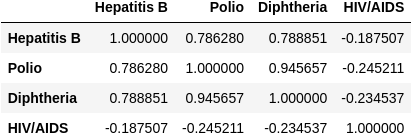
\includegraphics[width=0.35\textwidth]{img/1.png}
            	\caption{Matriz de correlación Hepatitis B, Polio, Diphtheria, HIV/AIDS.}
            	
            	\label{fig:1}
            \end{figure}
            
            Se ve una muy alta correlación entre Polio y Diphtheria y, a su vez, una considerablemente alta entre las mencionadas anteriormente y Hepatitis B. HIV/AIDS no tiene correlación con las demás, como esperábamos.
            
            
            Empecemos analizando las distribuciones de Hepatitis B, Polio y Diphtheria mediante un Boxplot que se ve en la Figura \ref{fig:2} y mediante histogramas como se ve en la Figura \ref{fig:3}.
            
             \begin{figure}[H]
            	\centering
            	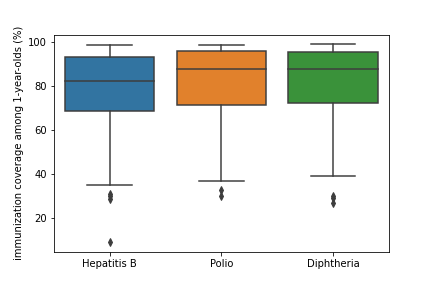
\includegraphics[width=0.35\textwidth]{img/2.png}
            	\caption{Boxplot Hepatitis B, Polio, Diphtheria.}
            	Se observan distribuciones muy parecidas en los tres casos.
            	\label{fig:2}
            \end{figure}
            
                    
               \begin{figure}[H]
              \centering
              \begin{subfigure}{0.3\linewidth}
                \centering
                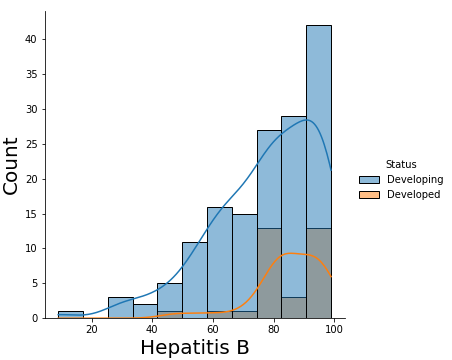
\includegraphics[width=\textwidth]{img/3.png}
              \end{subfigure}
              \hfill
                \begin{subfigure}{0.3\linewidth}
                \centering
                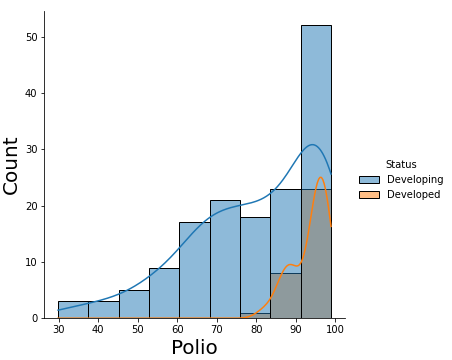
\includegraphics[width=\textwidth]{img/4.png}
              \end{subfigure}
                \hfill
                \begin{subfigure}{0.3\linewidth}
                \centering
                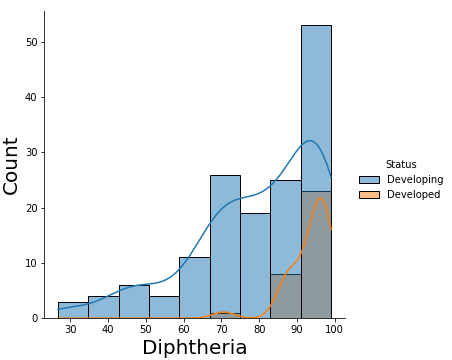
\includegraphics[width=\textwidth]{img/5.png}
              \end{subfigure}
               \caption{Histogramas Hepatitis B, Polio, Diphtheria.}
               \label{fig:3}
        \end{figure}

         En conclusión, Diphtheria, Polio y Hepatitis B tienen distribuciones muy similares y con una alta correlación, lo que nos permitiría unificarlas o descartar algunas de ellas de ser necesario.
         
         
         Se ve que en general, los países suelen tener un alto porcentaje de vacunados. Sin embargo, se ven casos atípicos en lo que esto no sucede; creemos que esto tendrá un impacto visible en la expectativa de vida.   
         
        Ahora, veamos el aspecto de la variable HIV/AIDS mediante un Boxplot e Histograma como se ve en la Figura \ref{fig: 4}.    
        
              
               \begin{figure}[H]
              \centering
              \begin{subfigure}{0.5\linewidth}
                \centering
               Tipo 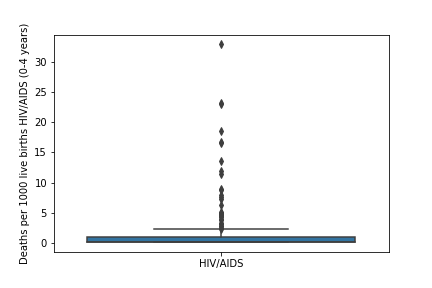
\includegraphics[width=\textwidth]{img/7.png}
              \end{subfigure}
              \hfill
                \begin{subfigure}{0.4\linewidth}
                \centering
                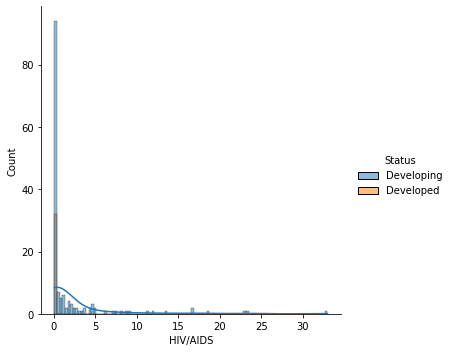
\includegraphics[width=\textwidth]{img/6.png}
              \end{subfigure}
               \caption{Distribución HIV/AIDS.}
               \label{fig: 4}
               
        \end{figure}
        
        Se ve que la mayoría de los países se concentran en alrededor de 0 a 5 muertes. Sin embargo, también podemos destacar la presencia de unos pocos outliers, que representan países con más casos, llegando a un máximo de alrededor de 30, los cuales creemos que tendrán un impacto en la expectativa de vida de estos países. Es notable que todos los países que tienen más de 5 muertes se encuentran en África. Esto podría explicarse en parte por la delicada situación económica de este continente, pero también por ser allí donde surgió esta enfermedad. 

       Veamos como se relaciona Life expectancy con estas variables, primero reportamos el coeficiente de correlación:
       
       \begin{verbatim}
            Hepatitis B        0.424982
            Polio              0.679231
            Diphtheria         0.672322
            HIV/AIDS          -0.587153
       \end{verbatim}
       
       Veamos mejor estas relaciones en la Figura \ref{fig: 5}. 
       
       
               \begin{figure}[H]
              \centering
              \begin{subfigure}{0.2\linewidth}
                \centering
                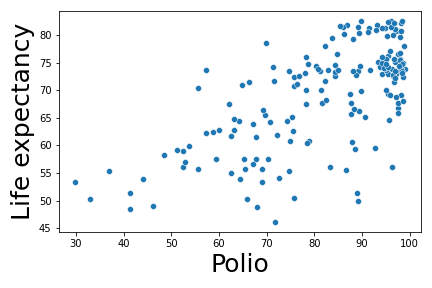
\includegraphics[width=\textwidth]{img/9.png}
              \end{subfigure}
              \hfill
                \begin{subfigure}{0.2\linewidth}
                \centering
                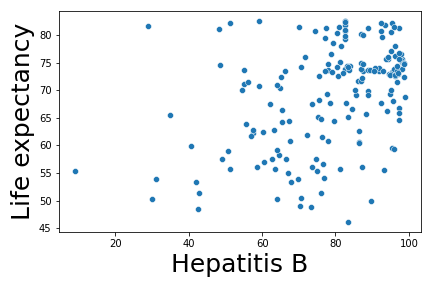
\includegraphics[width=\textwidth]{img/10.png}
              \end{subfigure}
              \hfill
                \begin{subfigure}{0.2\linewidth}
                \centering
                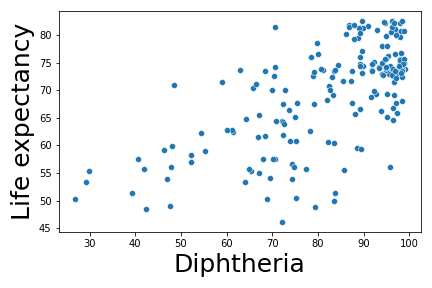
\includegraphics[width=\textwidth]{img/11.png}
              \end{subfigure}
                \hfill
                \begin{subfigure}{0.2\linewidth}
                \centering
                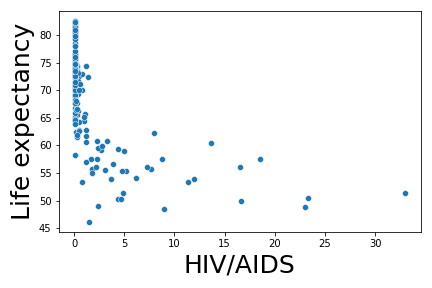
\includegraphics[width=\textwidth]{img/8.png}
              \end{subfigure}
               \caption{Scatterplot enfermedades VS Life expectancy.}
               	
               \label{fig: 5}
        \end{figure}
    \end{itemize}

Se ve que, como pensábamos, cuantos más vacunados hay, mayor es la expectativa de vida para las tres primeras y, cuantas más muertes se reportan, menor será la expectativa de vida en el caso de HIV/AIDS.

\subsection{Indicadores económicos: PBI, Composición del Ingreso, Gasto en Salud}
% Status	percentage expenditure	Total expenditure	GDP	Income composition of resources
    \begin{itemize}
        \item Datos faltantes
        
            Total expenditure tiene 2 NaNs, GDP 25 e Income composition of resources 10. Consideramos adecuado reemplazarlo por la mediana resultante para cada característica individual.
            
        \item Tipo de datos
        
            Status es una variable categórica, percentage expenditure en realidad no está reportando un porcentaje, encontramos valores mayores a 100, por lo que lo descartaremos.
            Total expenditure es un porcentaje, GDP es una variable numérica e Income composition of resources es otra variable numérica acotada del 0 al 1.  
            
        \item Distribución 
        
            Observemos la correlación entre las características previamente mencionados en la Figura \ref{fig: 6}.
            
              \begin{figure}[H]
            	\centering
            	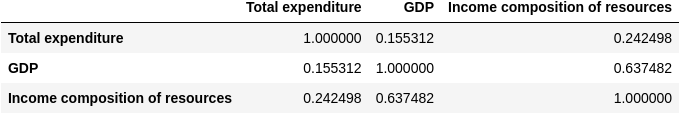
\includegraphics[width=0.50\textwidth]{img/12.png}
            	\caption{Matriz de correlación Total expenditure, GDP, Income composition of resources.}
            	No vemos una correlación muy significante entre ninguna de las características, aunque sí un poco más alta entre Income composition of resouces y GDP.
            	\label{fig: 6}
            \end{figure}
            
            Veamos si encontramos una relación entre las variables, más allá de la lineal, que nos ayude a interpretar nuestros datos en la siguiente Figura. 
            
               \begin{figure}[H]
              \centering
              \begin{subfigure}{0.3\linewidth}
                \centering
                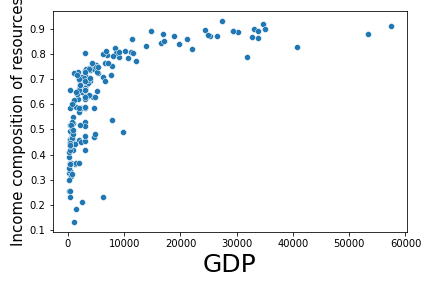
\includegraphics[width=\textwidth]{img/13.png}
              \end{subfigure}
              \hfill
                \begin{subfigure}{0.3\linewidth}
                \centering
                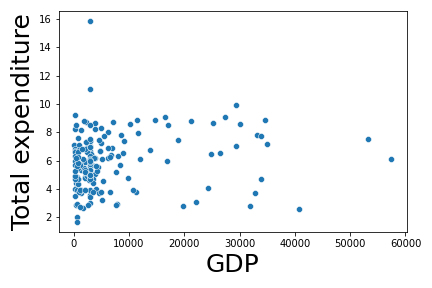
\includegraphics[width=\textwidth]{img/14.png}
              \end{subfigure}
                \hfill
                \begin{subfigure}{0.3\linewidth}
                \centering
                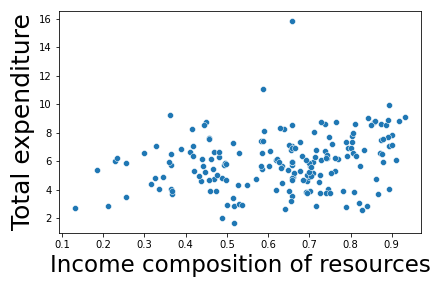
\includegraphics[width=\textwidth]{img/15.png}
              \end{subfigure}
               \caption{Scatterplots entre Total expenditure, GDP, Income composition of resources.}
               \label{fig: 7}

        \end{figure}

            En el primer gráfico se observa una relación particular entre GDP e Income composition of resources; si el GDP es muy bajo, el ICR puede tomar diversos valores, mientras que cuando el GDP es alto, el ICR también lo es, pero no podemos hablar de linealidad (se mantiene estático a partir de GDP = $20.000$ USD). Esto genera una curva de tipo exponencial.
            
            En el segundo y tercer gráfico no observamos nada que nos llame la atención, simplemente las variables están poco correlacionadas. Sin embargo, nos ayudan a entender las distribuciones de las variables; por ejemplo, podemos destacar que tanto Total expenditure como GDP tienen poca varianza, ya que vemos a todos los puntos concentrados en un espacio delimitado del gráfico b. De la misma manera se ve que ICR tiene mucha varianza.
            
            
            Para completar el análisis particular de estos datos, veamos sus respectivas distribuciones en la Figura \ref{fig: 8}.
            
            
                    
               \begin{figure}[H]
              \centering
              \begin{subfigure}{0.3\linewidth}
                \centering
                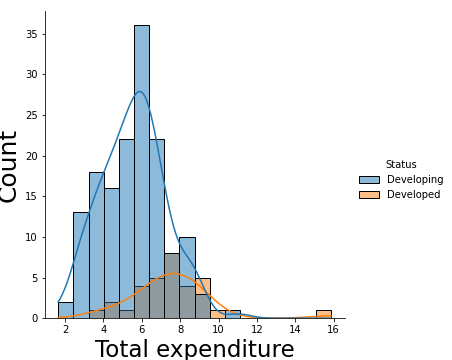
\includegraphics[width=\textwidth]{img/16.png}
              \end{subfigure}
              \hfill
                \begin{subfigure}{0.3\linewidth}
                \centering
                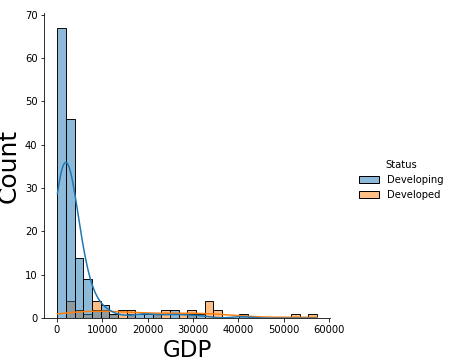
\includegraphics[width=\textwidth]{img/17.png}
              \end{subfigure}
                \hfill
                \begin{subfigure}{0.3\linewidth}
                \centering
                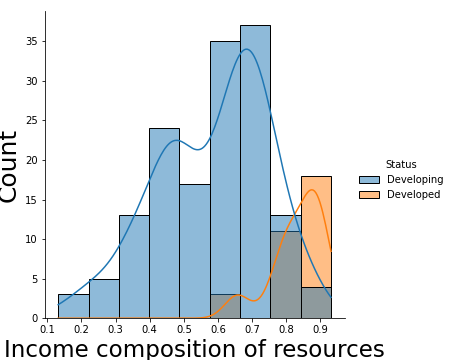
\includegraphics[width=\textwidth]{img/18.png}
              \end{subfigure}
               \caption{Histogramas Total expenditure, GDP, Income composition of resources.}
               \label{fig: 8}
        \end{figure}
            
            
            
            Tanto la distribución de Total expenditure como la de ICR tienen forma de campana de Gauss, con sus picos en 6 y 0.6, respectivamente. El GDP, por otro lado, tiene forma hiperboloide. Como es de esperar, los tres indicadores suelen ser mayores en los países 'desarrollados'. 
            
            Creemos que ICR estará correlacionada directamente con la expectativa de vida, ya que el bienestar económico influye de diversas maneras en la expectativa de vida, tanto a nivel individual como colectivo.
            
            Por la misma razón, esperamos que GDP correlacione positivamente con la expectativa de vida. Sin embargo, es posible que en menor manera, ya que el ICR es un índice más complejo que tiene en cuenta más factores, algunos relacionados con la distribución del ingreso. 
            
            Por otro lado, creemos que Total expenditure debería correlacionar positivamente, pero dudamos respecto a la magnitud. El hecho de que esté en términos absolutos, independientemente del nivel de población que tenga el país, lo hace un indicador poco informativo.
            
            Observemos los datos de la correlación a continuación y veamos si las hipótesis son ciertas:
            
             \begin{verbatim}
            Total expenditure                  0.288134
            GDP                                0.572807
            Income composition of resources    0.777659
       \end{verbatim}
       
       Veamos mejor estas relaciones en la Figura \ref{fig: 9}. 
       
       
               \begin{figure}[H]
              \centering
              \begin{subfigure}{0.3\linewidth}
                \centering
                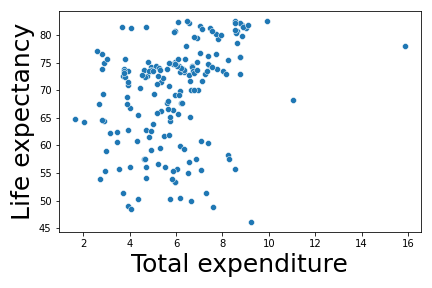
\includegraphics[width=\textwidth]{img/19.png}
              \end{subfigure}
              \hfill
                \begin{subfigure}{0.3\linewidth}
                \centering
                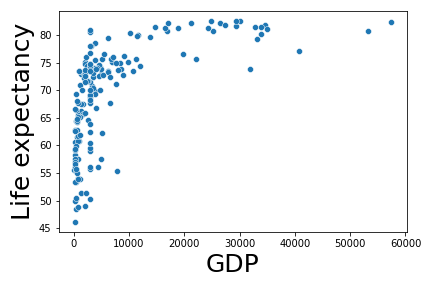
\includegraphics[width=\textwidth]{img/20.png}
              \end{subfigure}
              \hfill
                \begin{subfigure}{0.3\linewidth}
                \centering
                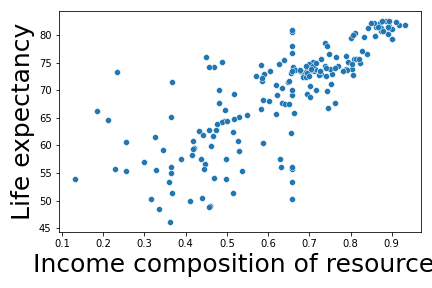
\includegraphics[width=\textwidth]{img/21.png}
              \end{subfigure}
               \caption{Scatterplot Life expectancy.}
               	
               \label{fig: 9}
        \end{figure}
  
    \end{itemize}
    
  Efectivamente podemos observar que prácticamente no existe correlación con Total expenditure. En cuanto a ICR y GDP, si bien tienen formas distintas, ambos cumplen una propiedad: un indicador alto garantiza una expectativa de vida alta, pero un indicador bajo no necesariamente implica lo contrario.  
  
\subsection{Indicadores Físicos: IMC, deladez entre 5-9 años y entre 1-19, consumo de Alcohol}   
% BMI, Alcohol   
\begin{itemize}
    \item Datos faltantes
    
    De BMI faltan dos. De alcohol falta uno. Estos campos serán completados utilizando la mediana de los mismos. De las variables thinness faltan dos en cada una.
    
    \item Tipo de datos
    
    Todas son variables numéricas. BMI es una métrica que relaciona el peso de un individuo con su altura ($\frac{peso}{altura^2}$). Los mismos están acotados. 
    
    Por otro lado, Alcohol representa el consumo \textit{per cápita} de alcohol puro en litros.
    
    Las variables thinness 5-9 y thinness 1-19 son un porcentaje.
    
    \item Distribución
    
    Calculamos el coeficiente de correlación entre estas variables y obtuvimos \texttt{0.504825}. 
    
    Para visualizar mejor la relación entre variables hacemos scatterplots (Figura \ref{fig: 10})
    
    \begin{figure}[H]
              \centering
              \begin{subfigure}{0.2\linewidth}
                \centering
                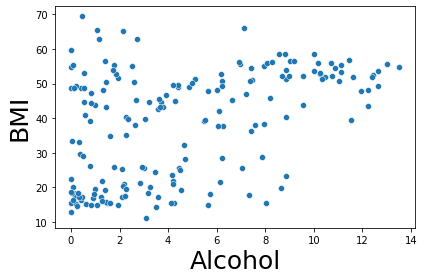
\includegraphics[width=\textwidth]{img/22.png}
              \end{subfigure}
              \hfill
                \begin{subfigure}{0.2\linewidth}
                \centering
                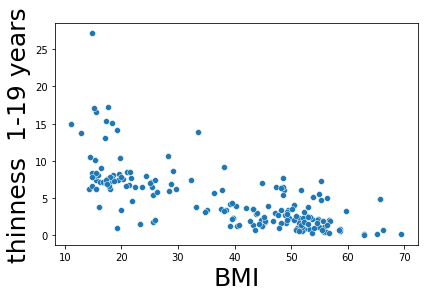
\includegraphics[width=\textwidth]{img/27.png}
              \end{subfigure}
                \hfill
                \begin{subfigure}{0.2\linewidth}
                \centering
                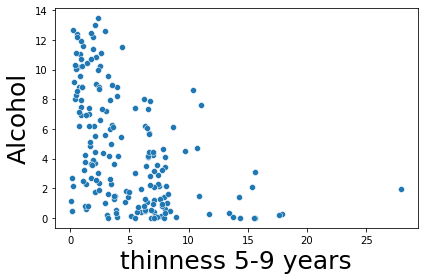
\includegraphics[width=\textwidth]{img/28.png}
              \end{subfigure}
                            \hfill
                \begin{subfigure}{0.2\linewidth}
                \centering
                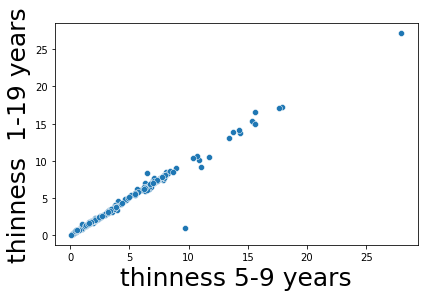
\includegraphics[width=\textwidth]{img/29.png}
              \end{subfigure}
               \caption{Scatterplots.}
               \label{fig: 10}
        \end{figure}
    
    En primer lugar, ambas variables thinness están fuertemente relacionadas, parecen prácticamente iguales. Esto tiene sentido, dado que indican lo mismo en distintas grupos demográficos, estando uno (5-9 años) incluido en el otro (1-19 años).  
    
    Por otro lado, vemos que BMI y thinness están inversamente relacionados; esto es porque lógicamente, un alto porcentaje de thinness implica un bajo BMI y viceversa.
    
    En cuanto a la característica alcohol, no se ve una correlación significante con ninguno de los demás.
    
    Ahora veamos la distribución de las mismas.
        
          \begin{figure}[H]
            \centering
              \begin{subfigure}{0.2\linewidth}
                \centering
                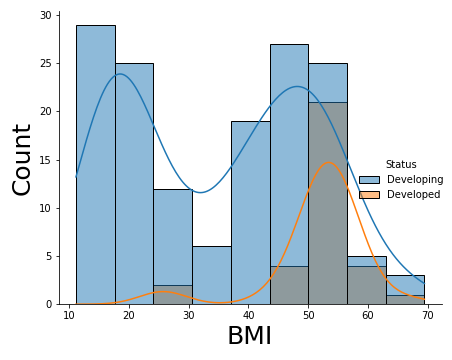
\includegraphics[width=\textwidth]{img/23.png}
              \end{subfigure}
              \hfill
                \begin{subfigure}{0.2\linewidth}
                \centering
                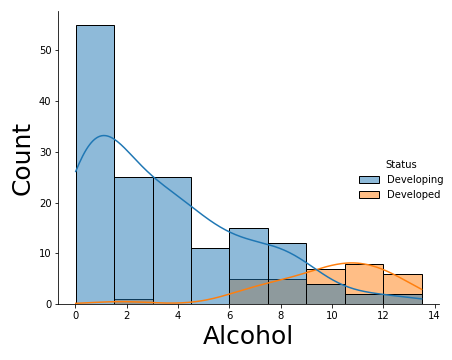
\includegraphics[width=\textwidth]{img/24.png}
              \end{subfigure}
              \hfill
                \begin{subfigure}{0.2\linewidth}
                \centering
                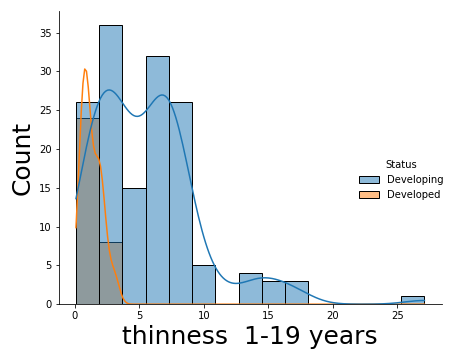
\includegraphics[width=\textwidth]{img/25.png}
              \end{subfigure}
                \hfill
                \begin{subfigure}{0.2\linewidth}
                \centering
                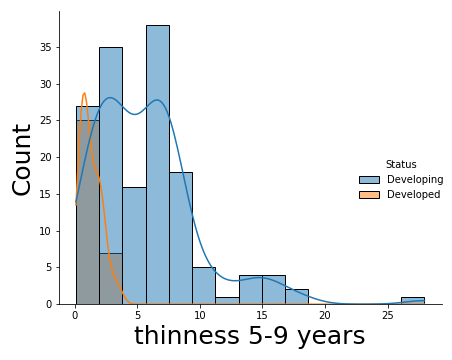
\includegraphics[width=\textwidth]{img/26.png}
              \end{subfigure}
               \caption{Distribución.}
               
               \label{fig: 17}
        \end{figure}
        
        BMI posee una distribución bimodal. Notemos que el BMI no debe tomar valores extremos, y que hay un intervalo óptimo en el cuál el coeficiente debería estar. Por lo tanto, creemos que la expectativa de vida sera más baja en países cuyo BMI se encuentre por encima (obesidad) o por debajo (desnutrición) de este intervalo. Creemos que los picos se corresponden con desnutrición y obesidad respectivamente. En países Developed el pico de desnutrición es muy bajo.
        
        En el gráfico de Alcohol podemos observar que en países Developing hay mucho menos consumo que en países Developed. Imaginamos que, a grandes rasgos, cuanto mayor sea el consumo de alcohol promedio, menor será la expectativa de vida, debido a los efectos del mismo sobre la salud.
        
        En cuanto a las variables de thinness, tal como se mencionó previamente, se ve la gran similitud entre ambas. Las mismas tienen, en países desarrollados, una gran concentración en valores cercanos a 0, y en países subdesarrollados hay dos picos: uno cercano a 0 y otro con valores más altos. Creemos que esto se debe a que dentro del grupo Developing entra una gran variedad de países con distintas realidades socio-económicas.
        
    Ahora veamos qué correlación tiene cada una de estas variables con Life expectancy.
    
          \begin{figure}[H]
            \centering
              \begin{subfigure}{0.2\linewidth}
                \centering
                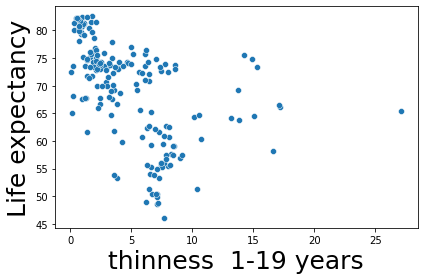
\includegraphics[width=\textwidth]{img/30.png}
              \end{subfigure}
              \hfill
                \begin{subfigure}{0.2\linewidth}
                \centering
                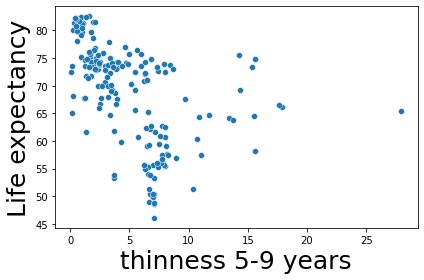
\includegraphics[width=\textwidth]{img/31.png}
              \end{subfigure}
              \hfill
                \begin{subfigure}{0.2\linewidth}
                \centering
                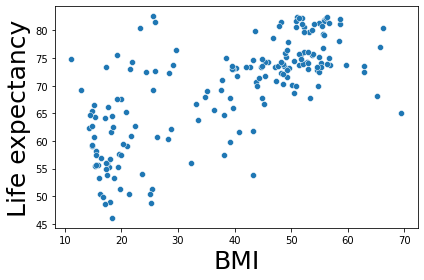
\includegraphics[width=\textwidth]{img/32.png}
              \end{subfigure}
                \hfill
                \begin{subfigure}{0.2\linewidth}
                \centering
                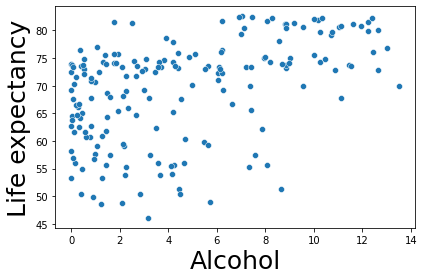
\includegraphics[width=\textwidth]{img/33.png}
              \end{subfigure}
               \caption{Scatterplots VS Life expectancy.}
               
               \label{fig: 18}
        \end{figure}    
    
    En los gráficos de las variables thinness (que son casi idénticos) se ve una relación inversa: a mayor thinness, menor Life expectancy. 
    Era esperable, dado que un bajo peso suele ser indicador de una nutrición precaria, lo que afecta gravemente a la salud (además de que la desnutrición puede entenderse como consecuencia de una situación socio-económica complicada, que también afecta a la expectativa de vida). 
    Resultados similares se observan con BMI.

    
    Alcohol presenta una leve correlación directa. Esto fue en contra de nuestras predicciones. Sin embargo, volviendo a observar los datos podemos entender que este efecto se puede deber a la correlación entre el consumo de alcohol y la riqueza de un país (en particular se observó que los países desarrollados consumen más alcohol que aquellos en vías de desarrollo).
    
    
    Veamos ahora los coeficientes de correlación obtenidos:
    
    \begin{verbatim}
   		
      thinness 1-19 years   -0.514356
      thinness 5-9 years    -0.507002
      BMI                   0.712117
      Alcohol               0.460338
    \end{verbatim}
    
    Entre éstas variables, la que presenta más correlación es BMI. 
\end{itemize}

%%%%%%%%%%%%%%%%%%%%%%%%%%%%%%%%%%%%%%%%%%%%%%%%%%%%%%%%    
    
\subsection{Otros indicadores: Mortalidad Adulta, Infantil, Escolarización y Población}

% Adult mortality: Adult Mortality Rates of both sexes (probability of dying between 15 and 60 years per 1000 population)

%- Infant deaths: Number of Infant Deaths per 1000 population

%- under-five deaths: Number of under-five deaths per 1000 population

%- Population: Population of the country

%- Schooling: Number of years of Schooling(years)



\begin{itemize}
    \item Datos faltantes
    
    De Population faltan 30 datos, y de Schooling faltan 10. Los reemplazamos por la mediana. El resto de las variables tiene todos sus datos presentes.
    
    \item Tipo de datos
    
    Todas son variables numéricas. Adult mortality, Infant deaths y under-five deaths representan cuántas muertes por cada 1000 personas ocurren según cada grupo etario.  Population es simplemente la población del país, y Schooling es la cantidad de años de escolaridad promedio.
    
    \item Distribución
    
    Para visualizar la correlación entre variables haremos scatterplots (Figura \ref{fig: 13})
    
    \begin{figure}[H]
              \centering
              \begin{subfigure}{0.15\linewidth}
                \centering
                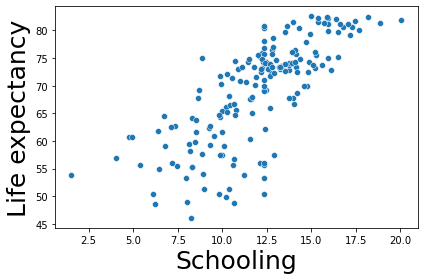
\includegraphics[width=\textwidth]{img/34.png}
              \end{subfigure}
              \hfill
                \begin{subfigure}{0.15\linewidth}
                \centering
                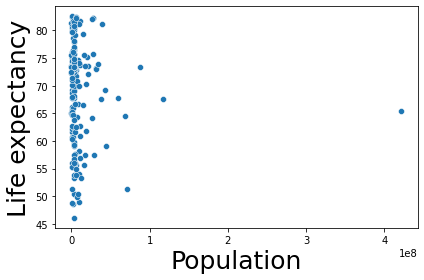
\includegraphics[width=\textwidth]{img/35.png}
              \end{subfigure}
                \hfill
                \begin{subfigure}{0.15\linewidth}
                \centering
                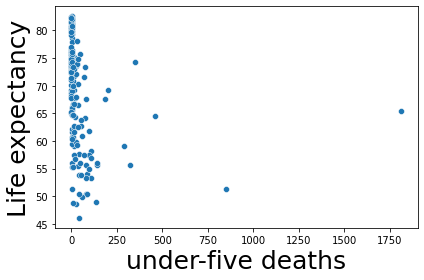
\includegraphics[width=\textwidth]{img/36.png}
              \end{subfigure}
                            \hfill
                \begin{subfigure}{0.15\linewidth}
                \centering
                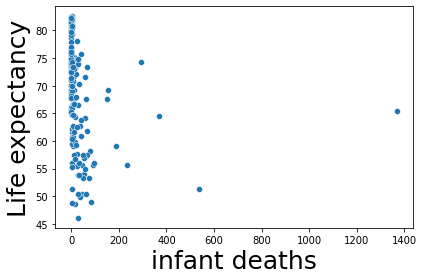
\includegraphics[width=\textwidth]{img/37.png}
              \end{subfigure}
                          \hfill
                \begin{subfigure}{0.15\linewidth}
                \centering
                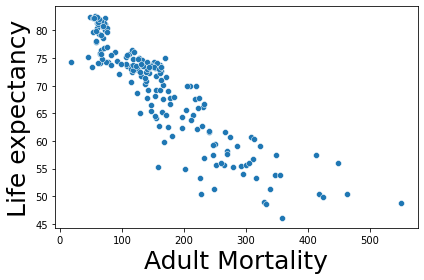
\includegraphics[width=\textwidth]{img/38.png}
              \end{subfigure}
               \caption{Scatterplots.}
               \label{fig: 13}
        \end{figure}

   Se ve una muy alta correlación con Schooling, lo que resulta lógico debido a que más años de educación parecerían indicar una mejor calidad de vida.
   
   Por otro lado, Population claramente no tiene ningún tipo de asociación con Life expectancy. 
   
   under-five deaths e infant deaths se comportan de una manera que no esperábamos; intuitivamente creeríamos que la mortalidad infantil esta muy correlacionada con la expectativa de vida. Sin embargo, eso no está sucediendo con nuestros datos; nos damos cuenta de que la razón de esto es porque los datos parecen estar mal.
   
   Se ven datos mayores a 1750 muertes cada 1000 habitantes, lo que no tiene sentido y nos lleva a descartar ambas características. Aunque reportar este error antes nos hubiese ahorrado algo de tiempo, nos damos cuenta del poder de un data-explore.
   
   
    Ahora veamos la distribución de Schooling, Population y Adult Mortality.
        
          \begin{figure}[H]
            \centering
              \begin{subfigure}{0.3\linewidth}
                \centering
                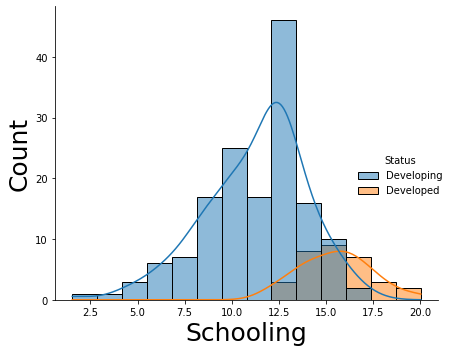
\includegraphics[width=\textwidth]{img/39.png}
              \end{subfigure}
              \hfill
                \begin{subfigure}{0.3\linewidth}
                \centering
                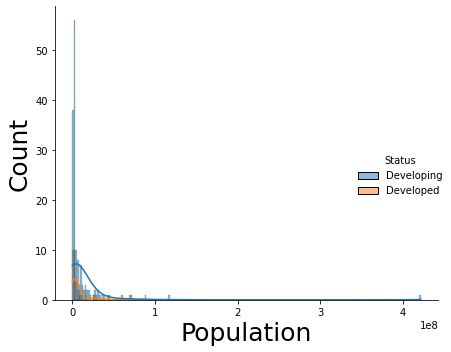
\includegraphics[width=\textwidth]{img/40.png}
              \end{subfigure}
              \hfill
                \begin{subfigure}{0.3\linewidth}
                \centering
                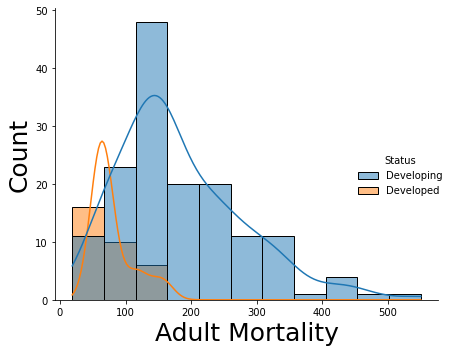
\includegraphics[width=\textwidth]{img/41.png}
              \end{subfigure}
               \caption{Distribución.}
               
               \label{fig: 17}
        \end{figure}
        
Tanto para Schooling y Adult Mortality se observan curvas normales y para los países desarrollados se observa más cantidad de años escolares y menos mortalidad en adultos que para los sub-desarrollados. 
 
En cuanto a Population, se observa una curva esperable. Sin embargo, no creemos que este dato nos sea de mucha utilidad.        
     
\end{itemize}    
    
    
    
% Podría hacerse mientras se hace sección 6. \subsubsection{Relación entre enfermedades, causas y consecuencias}
   
\newpage
\section{Relacionando expectativa de vida con regresores}

\subsection{Analisis General}
Vamos a querer predecir la expectativa de vida utilizando Cuadrados Mínimos Lineales con distintos regresores. Observamos la tabla de correlación de las variables para tener una idea de cuáles regresores serán más útiles para el modelo, intentando elegir los que mejor se relacionen a la expectativa de vida y a su vez tengan poca correlación entre ellos.


 \begin{figure}[H]
	\centering
	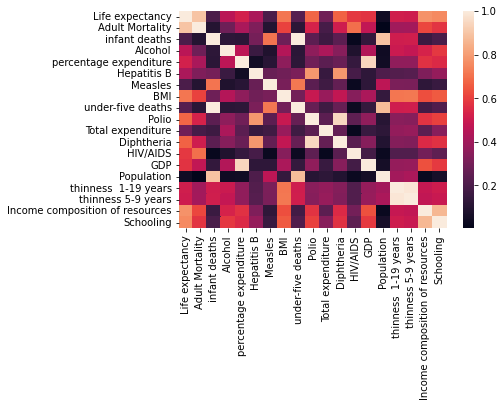
\includegraphics[width=0.7\textwidth]{img/heatmap_corr.png}
	\caption{Heatmap de la matriz de correlación de las variables (en valor absoluto).}
	\label{heatmap}
\end{figure}
        
Viendo la Figura \ref{heatmap} podemos  obtener una primera intuición sobre cuáles variables funcionarán mejor como regresores y cuáles no aportarán mucho al modelo. En principio podemos ver que variables como Adult Mortality e Income composition of resources están muy relacionadas a Life expectancy y serán buenos predictores, mientras que otras como Population, Measles e infant deaths no parecen aportar mucho.
 \begin{figure}[H]
	\centering
	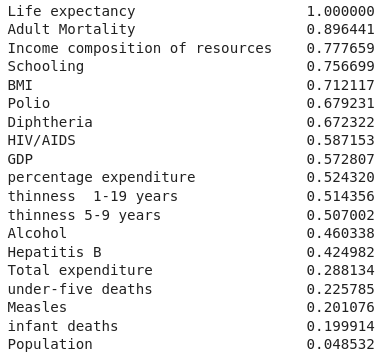
\includegraphics[width=0.45\textwidth]{img/life_exp.png}
	\caption{Correlación entre cada variable y Life Expectancy}
	\label{corr}
\end{figure}

En la Figura \ref{corr} podemos ver cuáles son las variables que más explican la expectativa de vida. Nos interesará elegir algunas de estas variables para la predicción, intentando mejorar las distintas métricas pero a la vez usando la menor cantidad de regresores posibles, buscando disminuir la multicolinealidad. Para eso será necesario tener la menor correlación posible entre las variables utilizadas. Además para la elección de los regresores tendremos en cuenta algunas métricas útiles como el R2 ajustado, el RSE y el VIF para medir la colinealidad. Notamos que usamos los datos normalizados, restando a cada regresor su media y dividiéndolo por su desvío estándar. También agregamos una nueva variable logGDP.


\subsubsection{V1}

Para nuestra primera versión del modelo observamos las variables que están más relacionadas a la expectativa de vida. Comenzamos con un solo regresor y luego vemos cómo mejora el modelo agregando más variables. Para empezar utilizamos Income composition of resources que es una de las variables más relacionada a expectativa de vida. No utilizamos Adult Mortality porque la mortalidad adulta como concepto se relaciona de manera muy directa con la expectativa de vida y nos parece más interesante la relación con Income Composition que tiene en cuenta diversas variables económicas de los países.

Para nuestra primer regresor observamos como dan las métricas con las variables que vimos que están mas correlacionadas a expectativa de vida. Esperamos que Income composition of resources sea de los mejores predictores ya que es el que tiene mayor correlación. Efectivamente el que obtuvo mejores métricas fue el Income composition of resources, con los siguientes valores:

Income composition of resources:

R2: [0.60475395]
R2 ajustado: [0.60257027]
RSE: [5.79131289]



\subsubsection{V2}

En la segunda iteración nos interesa agregar otro regresor que explique mejor el modelo y mejore las métricas, en lo posible incrementando el R2 ajustado y disminuyendo el RSE, y que tenga poco VIF. Observando las variables vemos que la siguientes variables mas relacionadas a Life Expectancy son logGDP y Schooling, pero también sabemos que Income Composition of Resources y Schooling tienen alta correlación por lo que es probable que Schooling no aporte mucho al modelo. De hecho, el VIF entre estas dos variables es de 3.9476, bastante alto. Tiene sentido, considerando que los países con mayor bienestar económico tendrán mejores posibilidades para brindar acceso a la educación. Efectivamente vemos que al agregar Schooling obtenemos un R2 ajustado de 0.629. Por otra parte logGDP devuelve un R2 ajustado de 0.65 y un VIF de 2.954 que también es bastante alto.

Con las variables BMI, Polio, y Diphtheria obtenemos valores de VIF (calculados por separado, junto al ICR) de [1.66, 1.49 y 1.437 son los de Difteria, Polio, Hep B; respectivamente]; y de R2 ajustado 0.682, 0.681 y 0.686. Estos valores no están tan mal pero tampoco mejoran mucho el R2 ajustado.

A diferencia de con estas variables, el IRC tiene poca correlación con el indicador HIV/AIDS: el VIF da 1.098. A su vez, el modelo incorporando a esta variable mejora su R2 ajustado hasta el valor de 0.7399. Por un lado, vemos que incorporar este feature, aunque tenga menos correlación con la expectativa de vida que otras (como Schooling, BMI, etc.), aumenta en mayor medida el R2 ajustado. Esto se explica justamente por la baja colinealidad entre ella e IRC. Queda como una pregunta abierta cuál es específicamente la información que agrega esta variable al modelo. No creemos que la cantidad de muertos por VIH/SIDA sea tan grande como para afectar en sí misma a la expectativa de vida de forma significativa. Entonces, debe ser expresión de un fenómeno que sí la afecte notoriamente. Por lo visto anteriormente, parece no estar tan relacionado con el bienestar económico. Quedará pendiente para futuras investigaciones.   

% Algo interesante sucede agregando la variable HIV/AIDS, obteniendo un R2 ajustado de 0.739, a pesar de que HIV/AIDS tiene menos correlación con Life Expectancy que las variables ya mencionadas. Esto se puede explicar debido a que la correlación entre Income Composition y HIV/AIDS es menor que con las otras variables, por lo que el uso de HIV/AIDS aporta información útil al modelo con menor colinealidad. 

Predictor: ['Income composition of resources', 'HIV/AIDS']

Resultados de las métricas:

R2: 0.74276834

R2 ajustado: 0.73991021

RSE: 4.67202835

VIF: 1.0983151726267792

\subsubsection{Vn}

En iteraciones subsiguientes vamos a querer seguir agregando variables que estén poco relacionadas a los regresores ya utilizados y que a su vez se relacionen de alguna manera con la expectativa de vida. Por ejemplo, agregando Polio o Diphtheria el R2 ajustado aumenta al 0.802, 0.807. Observamos que agregar ambas variables (Polio y Diphtheria) no será muy útil ya que tienen alta correlación, y efectivamente vemos que obtenemos un R2 ajustado de 0.807 que es equivalente a agregar sólo Diphtheria. La siguiente variable que parece mejorar las métricas es BMI obteniendo un R2 ajustado de 0.834 y un VIF razonable de 1.804. Luego de esto no mejora mucho el R2, a los sumo agregando percentage expenditure que obtenemos un R2 ajustado de 0.8487350 y además obtenemos un menor VIF de 1.491986.
A partir de esta ultima inclusión no encontramos beneficio en agregar más variables ya que en todos los casos las métricas empeoraron o se mantuvieron iguales, probablemente porque están relacionadas a los regresores ya utilizados y no tengan mucho para aportar al modelo.

Un predictor final podría ser:
['Income composition of resources', 'HIV/AIDS', 'Diphtheria', 'BMI', 'percentage expenditure']


Resultados de las métricas:

R2: [0.8528907]

R2 ajustado: [0.84873507]

RSE: [3.53316018]

VIF: 1.491986365304516

\subsection{Análisis Por Categorias: Developing}

Observamos que podemos partir nuestro dataset en dos grandes grupos: países desarrollados y países en vías de desarrollo, y que esta división probablemente sea útil para el análisis de regresores. Partimos el dataset en dos y observamos sus características, comenzando con los países en vías de desarrollo.

 \begin{figure}[H]
	\centering
	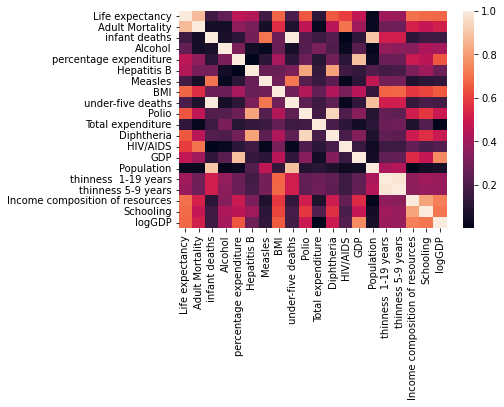
\includegraphics[width=0.7\textwidth]{img/heatmap_corr_developing.png}
	\caption{Heatmap de la matriz de correlación de las variables en países en vías de desarrollo (en valor absoluto).}
	\label{heatmap_developing}
\end{figure}

 \begin{figure}[H]
	\centering
	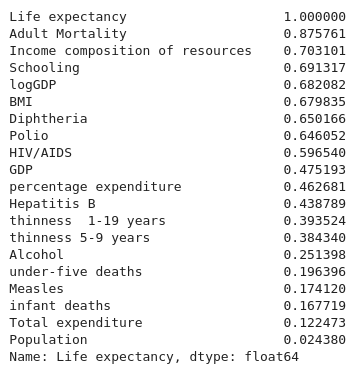
\includegraphics[width=0.5\textwidth]{img/tabla_developing.png}
	\caption{Tabla de correlaciones en países en vías de desarrollo.}
	\label{tabla_developing}
\end{figure}

A simple vista podemos ver que en términos generales el modelo es bastante parecido al utilizado en el caso general, esto puede deberse a que los países en vías de desarrollo son mayoría y por eso se parece mucho al caso global. Esperamos ver resultados mas particulares en el análisis de países desarrollados.

\subsubsection{V1}

Como primer regresor eligiremos al que tenga mejores métricas y explique mejor a la expectativa de vida. Comparamos las métricas R2/R2 ajustado y RSE entre las variables mas relacionadas con expectativa de vida y obtenemos de vuelta a Income composition of resources como el mejor regresor.

Income composition of resources:

R2: [0.49435129]
R2 ajustado: [0.49095768]
RSE: [6.15956382]

Observamos que comparado con el caso general, ahora ICR no explica tan bien al modelo (R2 de [0.60475395] a [0.49435129] y RSE de 5.7 a 6.15) lo cual tiene sentido ya que en la tabla de correlaciones vemos que la correlacion también es menor (de 0.77 a 0.70.)

\subsubsection{V2}

En la segunda iteración observamos que variable podemos agregar que mejore las métricas y ayude a explicar el modelo. Analizando las variables mas importantes (las mas relacionadas a expectativa de vida) sucede algo parecido al caso de análisis general donde la variable que mejora mas las métricas es HIV/AIDS con un R2 ajustado de 0.676, un RSE de 4.89 y un VIF de 1.06. Esto es interesante ya que en este caso HIV/AIDS es la variable numero 8 en término de relación con expectativa de vida, pero al estar muy poco relacionada con Income composition of resources es la que mejor explica el modelo. Por ejemplo, ICR y Schooling (la segunda mas relacionada a life exp) tiene R2 ajustado de 0.528, RSE de 5.9 y VID de 3.024, lo cual era esperable porque ICR y Schooling estan altamente relacionadas, por lo que un segundo predictor podría teniendo en cuenta ICR y HIV/AIDS

% Algo interesante sucede agregando la variable HIV/AIDS, obteniendo un R2 ajustado de 0.739, a pesar de que HIV/AIDS tiene menos correlación con Life Expectancy que las variables ya mencionadas. Esto se puede explicar debido a que la correlación entre Income Composition y HIV/AIDS es menor que con las otras variables, por lo que el uso de HIV/AIDS aporta información útil al modelo con menor colinealidad. 

Predictor: ['Income composition of resources', 'HIV/AIDS']

Resultados de las métricas:

R2: [0.53510995]

R2 ajustado: [0.52882765]

RSE: [5.9060978]

VIF: 3.024119900228316

\subsubsection{Vn}
En las siguientes iteraciones hacemos un proceso similar para ir agregando regresores, viendo en cada caso cual ayuda a explicar mejor el modelo buscando la menor correlacion entre los regresores y evitando la multicolinealidad (manteniendo un VIF bajo, al menos \< 5). En la búsqueda del tercer regresor encontramos los mejores resultados agregando Diphtheria y en el 4to agregando BMI, obteniendo un R2 ajustado de 0.81, un RSE de 3.723 y un VIF de 1.6265. Finalmente analizando un quinto regresor vemos que quizás se podría agregar percentage expenditure con un R2 ajustado de 0.8167, un RSE de 3.64 y un VIF de 1.373, pero comparando con la 4ta iteración vemos que no mejoran mucho las métricas por lo que un predictor final podría utilizar ICR, HIV/AIDS, Diphtheria, y BMI.

Predictor:
['Income composition of resources', 'HIV/AIDS', 'Diphtheria', 'BMI']

Metricas:

R2: [0.81519655]

R2 ajustado: [0.81013344]

RSE: [3.72375024]

VIF: 1.6265061009609258

\subsection{Análisis por Categorías: Developed}

Tomamos el conjunto de países desarrollados y observamos sus características. 

 \begin{figure}[H]
	\centering
	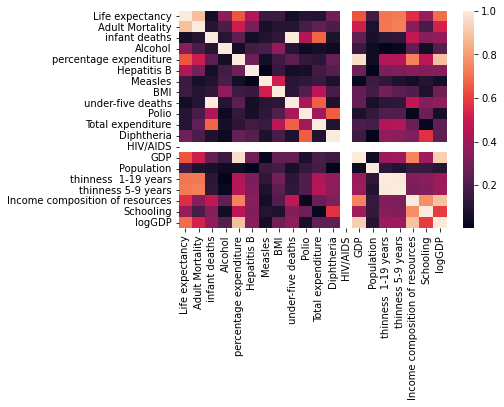
\includegraphics[width=0.7\textwidth]{img/heatmap_corr_developed.png}
	\caption{Heatmap de la matriz de correlación de las variables en países dessarrollados (en valor absoluto).}
	\label{heatmap_developed}
\end{figure}

 \begin{figure}[H]
	\centering
	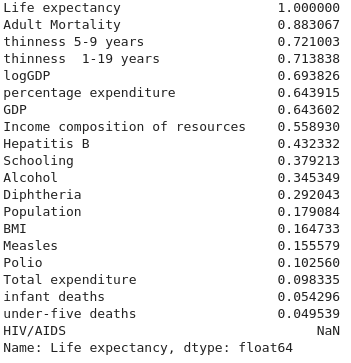
\includegraphics[width=0.4\textwidth]{img/tabla_developed.png}
	\caption{Tabla de correlaciones en países desarrollados.}
	\label{tabla_developed}
\end{figure}


A simple vista vemos que este modelo difiere bastante del análisis general y los países en vías de desarrollo. En primer lugar vemos un comportamiento extraño con la variable HIV/AIDS. Observando los datos vemos que todos los países desarrollados tienen el mismo valor de HIV/AIDS, y al aplicar la normalización de los datos se divide por el desvió estándar (que da 0) y obtenemos NaNs, por lo que desecharemos esta variable y no la tendremos en cuenta.

Podemos ver que hay algunas variables que toman un peso mucho mas importante en el caso de los países desarrollados: thinness 5-9 years y thinness 1-19 years. Sabemos que ambas están altamente correlacionadas por lo que tendremos en cuenta solo una. Nos pareció extraño ya que uno pensaría que en los países desarrollados no hay muchos casos de desnutrición, quizás pueda darse por algún problema regional de desnutrición. Vemos en los datos que los países con peores valores de thinness se encuentran en el este de Europa, países como Rumania, Latvia, Lituania y Bulgaria, esto puede deberse a una cuestión geográfica y también puede estar relacionado a problemas de pobreza y calidad de vida que no ocurren en países del oeste de Europa y se ven reflejados en el índice de desnutrición. 

\subsubsection{V1}

Como primer regresor elegimos thinness 5-9 years que es el que mejor explica la expectativa de vida. Observamos que en el futuro probablemente no agreguemos thinness 1-19 years ya que ambas están altamente correlacionadas. El resto de las variables (logGDP, percentage expenditure, GDP..) no dieron tan buenas métricas por lo que nos quedamos con thinness 5-9 years.

Predictor: ['thinness 5-9']

Metricas: 

R2: [0.51984568]

R2 ajustado: [0.50384054]

RSE: [2.27024552]

\subsubsection{V2}

Observamos las métricas tomando thinness 5-9 years y otras variables para ver cuales aportan mas información al modelo. El regresor con el que obtuvimos las mejores métricas fue logGDP obteniendo los siguientes resultados:

Predictor: ['thinness 5-9' y 'logGDP']

Metricas:

R2: [0.71880595]

R2 ajustado: [0.69941325]

RSE: [1.73734262]

VIF: 1.1833091879040005

\subsubsection{Vn}

En siguientes iteraciones encontramos como el mejor tercer regresor a la variable 'Alcohol' obteniendo valores de R2 ajustado = 0.74865007, RSE = 1.5610613 y 
VIF = 1.0573780269799327 y como cuarto regresor a la variable 'Measles' obteniendo valores de R2 ajustado = 0.75875508, RSE = 1.50180148 y VIF: 1.0506871. En búsqueda de un quinto regresor no encontramos ninguno que mejore las métricas, por lo que nos quedamos con los 4 regresores que tenemos. 

Predictor: ['thinness 5-9 years', 'logGDP', 'Alcohol', 'Measles']

Metricas:

R2: [0.78988346]

R2 ajustado: [0.75875508]

RSE: [1.50180148]

VIF: 1.0506871618402263

\section{Agregando información}
Una vez tenemos un buen modelo con los datos proporcionados, nos interesa agregar nuevos datos de otras fuentes que podrían complementar, y mejorar aun más las métricas previamente vistas.

La \href{https://www.who.int/data/gho/data/themes/mortality-and-global-health-estimates}{WHO} provee características distintas a las utilizadas en la experimentación hasta el momento, por lo que fue seleccionada como fuente. Una de ellas es la tasa de homicidios por cada 100000 habitantes\footnote{https://www.who.int/data/gho/data/indicators/indicator-details/GHO/estimates-of-rates-of-homicides-per-100-000-population}.

Es interesante poder analizar el impacto que las muertes no naturales por homicidio traen sobre la expectativa de vida general, así que se eligió para agregar al modelo ya definido.

Antes de poder utilizar los datos se tuvo que aplicar un proceso de limpieza de los mismos. Se analizo las columnas que el dataset tenia y lo que nos interesa de la misma. Las columnas que utilizamos fueron:
\begin{itemize}
    \item Period, el año del que provienen los datos de la medición.
    \item Dim1ValueCode, una variable categórica de 3 posibles valores.MLE(Male),FMLE(Female) y BTSX(Both sex).
    \item Location, el país al que corresponden los datos de la medición.
    \item FactValueNumeric, el valor promedio para la taza de homicidios.
\end{itemize}

El resto de las columnas tenían valores que aportaban poco una vez seleccionamos FactValueNumeric como el valor a usar(FactValueNumericLow,FactValueNumericHigh,Value). Columnas que tenían todos sus campos nulos, o repetidos. Y algunas que decidimos descartar porque ya estaban en los datos que teníamos(ParentLocation).

La manera en la que se limpiaron los datos fue la siguiente. Inicialmente, se eliminaron los datos con Period inferior a 2015, pues nuestro dataset en uso tiene en cada columna los promedios de los valores de cada año entre 2015 y la actualidad. Luego, nos quedamos con los valores Dim1ValueCode BTSX, dado que los datos de nuestro dataset no segregan por genero, y vamos a tener que unificarlos.Después de realizar los filtros mencionados nos quedamos con las columnas Location y FactValueNumeric. Se realiza un promedio entre las filas con la misma Location(los distintos años de la medición para ese país) y finalmente, se une al dataset original utilizando Location del dataset nuevo junto con Country del dataset original.

\begin{figure}[H]
              \centering
              \begin{subfigure}{0.5\linewidth}
                \centering
                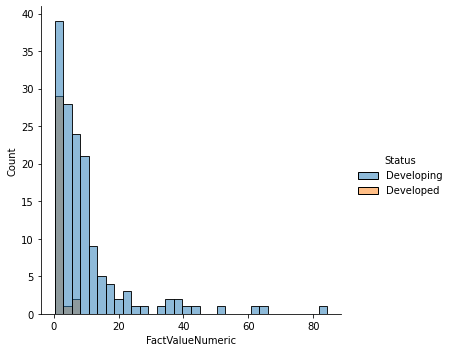
\includegraphics[width=\textwidth]{img/dist_homicides.png}
              \end{subfigure}
               \caption{Distribución de homicidios para países desarrollados y en vias de desarrollo.}
               \label{fig:dist_homicides}
        \end{figure}

En la figura \ref{fig:dist_homicides} podemos ver una distribución parecida a otras previamente vistas, como la figura \ref{fig: 4} para HIV/AIDS, solo que menos pronunciada en los primeros valores. Del mismo modo que la figura previamente mencionada, al separar entre Developing y Developed encontramos que la cantidad de suicidios para los países desarrollados es por mucho inferior a los no desarrollados, por lo que no aporta demasiado a este tipo de clasificación.
Como hipótesis respecto a esta característica se puede pensar que la tasa de homicidios va a tener algún tipo de influencia sobre la expectativa de vida, pues las muertes de causa no natural son un elemento categórico importante sobre las causas de muerte.

Para evaluarla, realizamos una ejecución de las métricas agregando a nuestro modelo mas completo la nueva característica.

Al ejecutar el predictor con la variable nueva se ve como el R2 ajustado empeora del 0.84873507 previo a 0.84787597, que, aun sin ser una disminución muy grande nos parecería indicar que no vale la pena agregarlo al predictor hasta este punto. Antes de descartar la característica decidimos aplicarle una función no lineal.

La función no lineal aplicada es logarítmica. Nuestra nueva característica mejora la predicción tanto para el R2 como el R2 ajustado, por lo que vale la pena conservarla en una nueva versión del mismo. El R2 pasa a ser de 0.8559576 y el ajustado de 0.85104706.

\begin{figure}[H]
              \centering
              \begin{subfigure}{0.5\linewidth}
                \centering
                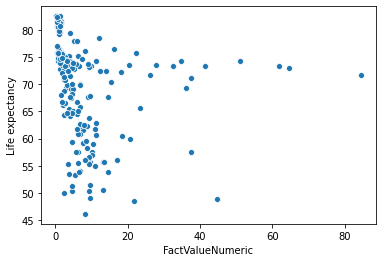
\includegraphics[width=\textwidth]{img/homicide_life_expectancy.png}
              \end{subfigure}
               \caption{Relación entre homicidios cada 1000 habitantes y expectativa de vida para un país.}
               \label{fig:life_expectancy_homicides}
        \end{figure}

Un posible motivo por el que nuestra característica responde mejor a una función logarítmica puede deberse a su relación con la expectativa de vida. En la figura \ref{fig:life_expectancy_homicides} podemos ver que  una expectativa de vida alta esta muy relacionada a una baja cantidad de homicidios, y al aumentar los mismos, la disminución de la expectativa de vida no es tan pronunciada.
\section{Análisis de outliers}

Antes de estudiar los coeficientes es necesario identificar, si es que los hay, aquellos países que pueden estar afectando a nuestro modelo en una manera no deseada por apartarse demasiado de los valores esperados.
Vamos a detectar outliers observando los gráficos de influencia (\textit{influence plots}) de los indicadores seleccionados.

Como se puede ver en el influence plot correspondiente al \textbf{Income Composition of Resources} (Figura \ref{fig:inf_icr}), no hay países que tengan valores medianamente altos de Leverage; es decir, no hay países que sean muy 'raros' en su valor de ICR. Algunos pueden tener un residuo studentizado medianamente alto, o una distancia de Cook no pequeña, pero al ser acompañados de Leverages bajos, no es necesario atenderlos.

\begin{figure}[H]
            \centering
             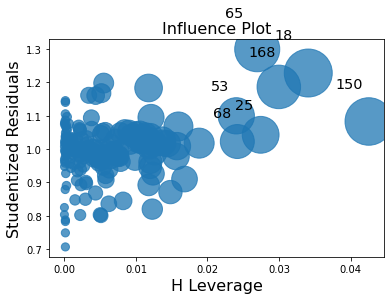
\includegraphics[scale = 0.5]{img/influ/icr.png}
             \caption{Influence plot correspondiente al ICR}
             \label{fig:inf_icr}
\end{figure}

Por otro lado, al analizar el gráfico relativo a \textbf{HIV/AIDS} podemos identificar un caso problemático.
El país con índice 155 (Suazilandia) exhibe a la vez valores altos en \textit{x}, en \textit{y} y en tamaño; es decir, tiene un valor 'raro' del indicador HIV/AIDS, es bastante distinto a lo predecible en su valor de Life Expectancy, y tiene mucho peso sobre el modelo.
Teniendo en cuenta este análisis, consideramos óptimo descartar la información que nos provee este país respecto a este indicador.
Más precisamente, reemplazamos su valor por la media. 
Con esta modificación el gráfico queda de la siguiente manera.

\begin{figure}[H]
            \centering
              \begin{subfigure}{0.45\linewidth}
                \centering
                \includegraphics[width=\textwidth]{img/influ/hiv.png}
              \end{subfigure}
              \hfill
                \begin{subfigure}{0.45\linewidth}
                \centering
                \includegraphics[width=\textwidth]{img/influ/hiv2.png}
              \end{subfigure}
             
               \caption{Influence plots para HIV/AIDS. A la izquierda, antes de modificar el valor de Swazilandia; a la derecha, después.}
               
               \label{fig:inf_hiv}
        \end{figure}
        
Continuando este análisis para \textbf{Diphtheria}, \textbf{BMI} y \textbf{percentage expenditure} no hallamos más outliers. En la Figura \ref{fig:inf_dift} se nota que los primeros dos manifiestan bajos valores sobre el eje \textit{x}. En el tercero también, excepto los países con índices 96 y 157. Estos países también exhiben una distancia de Cook considerable, pero no así la magnitud de los residuos studentizados. Por esto, no consideramos apropiado eliminar (o reemplazar el valor) de ninguno de estos elementos.  

\begin{figure}[H]
            \centering
              \begin{subfigure}{0.3\linewidth}
                \centering
                \includegraphics[width=\textwidth]{img/influ/difteria.png}
              \end{subfigure}
              \hfill
                \begin{subfigure}{0.3\linewidth}
                \centering
                \includegraphics[width=\textwidth]{img/influ/bmi.png}
              \end{subfigure}
              \hfill
                \begin{subfigure}{0.3\linewidth}
                \centering
                \includegraphics[width=\textwidth]{img/influ/percent_exp.png}
              \end{subfigure}
               \caption{Influence plots para Diphtheria (izq.), BMI (centro) y percentage expenditure (der.).}
               
               \label{fig:inf_dift}
        \end{figure}
        
\section{Análisis de coeficientes}
Ya con nuestro modelo final podemos realizar un ultimo análisis. Al aplicar cuadrados mínimos(sección \ref{sec:into_CML}) a un subconjunto de variables obtenemos un x$^*$. Este vector contiene los coeficientes que utilizamos en un nuevo conjunto de datos para obtener nuestro target.

Al utilizar x$^*$ en un dato para predecirlo lo que estamos haciendo es aplicar al feature i una multiplicacion por el valor x$^*_i$.Entonces, lo que ese particular valor nos dice es el peso que el feature i tiene sobre el calculo de la y predicha. La ultima posicion del vector no corresponde a ningun feature, es una variable independiente.

Entendiendo esto, vamos a analizar los valores de los coeficientes obtenidos en la ejecucion de nuestro ultimo modelo.


\begin{table}[H]
\centering
\begin{tabular}{ |p{4cm}||p{4cm}|  }
 \hline
 \multicolumn{2}{|c|}{Peso de coeficientes} \\
 \hline
 Coeficiente& Valor\\
 \hline
 Valor independiente   & 70.02485369\\
 Income composition of resources&2.64864459\\
 Diphtheria &2.46057022\\
 BMI    &2.06832015 \\
 percentage expenditure&1.08700785\\
 homicides(logaritmic)&-0.5486583\\
 HIV/AIDS&-2.97126444\\
 \hline
\end{tabular}
\caption{Tabla con coeficientes para cada caracteristica}
\label{fig:table_coef}
\end{table}


En la tabla \ref{fig:table_coef} podemos ver los valores de los coeficientes, ordenados de mayor a menor.
Como coeficiente de mayor valor tenemos la variable independiente, con una diferencia muy amplia respecto al resto. Esto nos podría estar indicando la cantidad de información que aun no podemos explicar en el modelo, que aun no tenemos característica a la que atribuirle ese peso.
Como siguiente coeficiente tenemos el income composition of resources, esto nos da un índice de desarrollo humano basado en el manejo de los recursos de la nación. Podemos entender esto como la variable que define mejor la expectativa de vida entre las presentadas. Esto puede deberse a lo que representa como métrica. Si es alto los ciudadanos de un país se ven beneficiados, y eso se traduce en una mayor expectativa de vida. El income composition of resources tiene en cuenta la economía de un país sin separarlo de la relación con sus ciudadanos.
Diphteria es la siguiente característica que fue priorizada por el modelo. El coeficiente es positivo, por lo que esto nos dice que países con un mayor grado de vacunación van a tener una mayor expectativa de vida que los que no lo tienen. Una cosa a notar es que la magnitud asignada al coeficiente es muy parecida a la de income composition of resources. Lo que nos indica es que la importancia de ambas características ara predecir la expectativa de vida son similares.
El BMI es un poco menos relevante en el calculo de la expectativa de vida que las características previas. Esto podría deberse a que hay un margen de peso para el cual la expectativa de vida se mantiene estable, y los extremos que la modifican.

Percentage expenditure esta fuertemente atado al GDP por lo que no tiene implicaciones tan directas sobre la expectativa de vida, pueden existir casos de países con GDP bajo y gasten muchos de sus recursos en salud, pero en términos económicos esos recursos sean menores a los gastados por un país con mayor GDP, utilizando un menor porcentaje del mismo.

Los coeficientes restantes son negativos, esto implicaría que todos ellos restan a la expectativa de vida, que tiene sentido al ver que son enfermedades o causas de muerte directa(homicidios).
La cantidad de homicidios tiene un coeficiente bajo, esto amerita mas analisis, pero a priori podemos adjudicarlo a la funcion aplicada. 
Quien mas afecta negativamente la expectativa de vida es el HIV/AIDS, esto puede deberse a su correlacion con falta de educacion sexual, que esta relacionada a la educacion en general y  podria relacionarse con la expectativa de vida.
\newpage
\section{Conclusiones}\label{sec:conclusiones}
A lo largo de este trabajo se logro percibir la dificultad de lograr una predicción precisa al empezar a manejar un modelo desconocido. Empezando con el análisis exploratorio, en el cual analizamos las diferentes características, y con ello, generamos nuestras primeras hipótesis. Luego, al utilizar el regresor y analizar su comportamiento fuimos capaces de reforzar nuestras afirmaciones o descartarlas. Tratamos con datos incompletos y cómo completarlos dependiendo de la existencia o no de una ``moda'' y tuvimos la oportunidad de agregar nueva información con intención de mejorar la predicción lograda hasta ese punto.
A partir del modelo que encontramos podemos concluir:

\begin{itemize}
    \item Los indicadores \textit{Polio}, \textit{Diphteria} y \textit{Hepatitis B } son redundantes entre sí (es decir, utilizar más de uno no suma información). Esto podría decirnos que son expresión de un mismo fenómeno. Como los tres son tasas de vacunación infantil, podemos concluir que alcanza con usar cualquiera de los tres como indicador de la vacunación infantil en general.
    
    \item Podemos utilizar \textit{IRC} y no \textit{GDP}. Como el primero está compuesto en parte por el segundo, esto nos muestra que el resto de los indicadores que lo componen aportan información relevante a fines de explicar la expectativa de vida, dándole valor agregado al modelo.
    
    \item \textit{BMI} es un buen indicador para sintetizar la información relativa a la nutrición (como \textit{thinness}, entre cualquier edad).
    
    \item Nos llama la atención la influencia que tiene el indicador \textit{HIV/AIDS}. No creemos que la cantidad de muertes por esta enfermedad sea tan grande como para afectar la expectativa de vida por sí sola. Intuimos que debe ser indicador de un fenómeno de mayor influencia, como pueden ser la dificultad en el acceso a la atención pediátrica o a la salud sexual y reproductiva, entre otros. Tambien notamos que el HIV AIDS puede ser indicador del desarrollo de los paises ya que todos los paises desarrollados tienen un indice HIV bajo y los no desarrollados tienen un indice HIV alto.
    
    \item Encontramos que puede resultar útil dividir al dataset en distintas categorias (Como Developed/Developing) para observar caracteristicas propias de los datos y encontrar predictores mas especificos para cada caso, por ejemplo observamos que en el caso general el indice de HIV es muy importante mientras que en el caso de paises desarrollados éste indice no aporta nada ya que todos los paises tienen un mismo indice HIV bajo y se puede descartar esta caracteristica.
\end{itemize}

Por otro lado, a lo largo de este trabajo analizamos la correlación entre distintas variables, buscando indicadores que expliquen satisfactoriamente la Expectativa de vida. Sin embargo, estas correlaciones no implican causalidad. Conocer cómo se dan las relaciones de causalidad entre las distintas variables que exploramos, y también otras que no incluimos, puede resultar de mayor interés. Carecemos de las herramientas para hacer ese análisis, por lo que quedará como trabajo futuro.

Analizamos los valores irregulares, o outliers de las características, la colinealidad y finalmente, los coeficientes obtenidos del modelo. Vimos la importancia de este mismo a la hora de entender el valor o peso que nuestras columnas seleccionadas tenían para la expectativa de vida.
\newpage
\bibliography{biblio}
\bibliographystyle{plainurl}
\end{document}